\chapter{The IceCube Experiment}
IceCube is a neutrino observatory located near the Amundsen-Scott South Pole Station close to the geographic South Pole. As already introduced in Section \ref{sec:detectors}, experiments that search for astrophysical neutrinos need enormous instrumented volumes. IceCube is the first gigaton neutrino detector ever built and was designed specifically for this case. It is buried beneath the surface of the Antarctic ice, starting from around 1450 meters and extending to a depth of about 2,500 meters ($\sim$300 meters above bedrock). The ice acts as a medium for both the interaction of a neutrino light propagation. In this chapter ..... Eigenlijk doe je dit een beetje verder\\ OVERAL HOOFDLETTERS VOOR CHAPTERS/SECTIONS/....
\newline
\noindent The main goal of the IceCube experiment is to learn more about the distant sources that we believe to be responsible for the detection of the highest-energy cosmic rays. As indicated in Section \ref{sec:neutrinos}, neutrinos are crucial in gaining information about these far away sources. Large-scale detectors are necessary to cover the faint flux of neutrinos with very high energies. Detecting the Cherenkov radiation (Chapter \ref{ch:cherenkov}) from neutrino interactions is the best way to observe these weakly interacting particles. As hadronic, elecromagnetic and muonic components from these interactions require a medium that has good light propagation charactaristics and extends to a couple of kilometers, the South Pole ice sheet acts as a near ideal component of the detector. As a proof of concept, the AMANDA (Antarctic Muon And Neutrino Detector Array) experiment was built to show that neutrinos with energies above 50 GeV could be detected in the Antarctic ice \cite{amandaurl,Andres:1999hm}. After construction was finalized, the detector was made up of 677 optical modules mounted on 19 separate strings that are spread out in a rough circle with a diameter of around 200 m. These strings were deployed by first ``drilling'' holes in the ice with a hot-water hose, showing that the technique works. After some years of data taking, it was clear that high-energy neutrinos could be observed, paving the way for the much bigger IceCube project \cite{Ahrens:2002gq}.


\begin{figure}
\centering
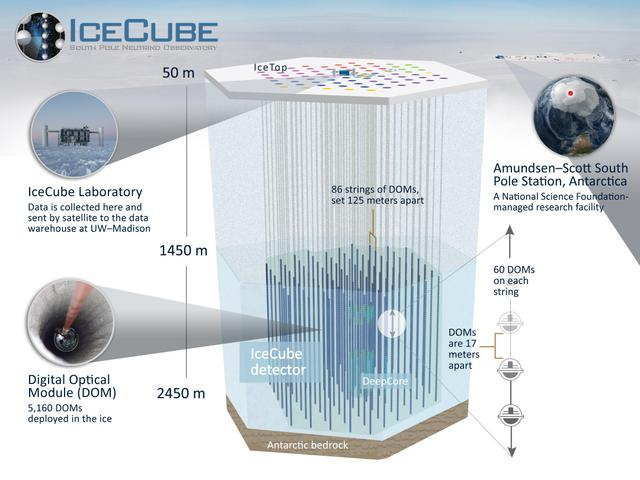
\includegraphics[width=1.1\textwidth]{chapter5/img/icecube_detector.jpg}
\caption{Illustration of the IceCube South Pole neutrino observatory.}
\label{fig:ICgeometry}
\end{figure} 

\section{Geometry}
The IceCube detector consists of three main parts that act as different purpose physics detectors. On the surface of the ice, water tanks with optical modules inside are spread out over an area of ??? and make up the \textit{IceTop detector}. This surface array was built as a cosmic ray detector and veto for the in-ice array. The \textit{in-ice IceCube} detector is the main component and consists of 4680 digital optical modules. In it's core, a denser subdetector, \textit{DeepCore}, significantly enhances the capabilities of the observatory in a limited volume. 480 sensors form the center of the DeepCore array. The three components combined make the facility a clear multipurpose physics detector. Figure \ref{fig:ICgeometry} shows the layout of the detector.

\subsection{In-Ice Array}
The in-ice array consists of 4680 digital optical modules (DOMs) that are able to register light that is scattered and propagated through the ice (more info about these modules can be found in Section \ref{subsec:doms}). The DOMs are attached to cables which are frozen vertically in the ice. In total, 78 of these ``strings'' were frozen into boreholes and arrayed over a cubic kilometer in a hexagonal shape. Because the ice is only transparent deep within, the DOMs are attached to the strings starting from a depth of 1450 meters to 2450 meters. Strings, as viewed from above, are spaced around 125 meters apart and along each string 60 DOMs are attached with a vertical separation of 17 meters. This design was chosen
in order to meet the primary science requirement of detecting astrophysical neutrinos in the energy range of $\mathcal{O}$(TeV)– $\mathcal{O}$(PeV).

In general, there are two event topologies that form the standard signatures of neutrinos in IceCube as indicated in Section \ref{sec:propagation}. \textit{Track-like events}, originating from charge-current muon neutrino interactions, provide an angular resolution at a typical angle of 1$^\circ$ for well contained and reconstructed tracks at 1 TeV and improves to $\sim 0.3^\circ$ for neutrinos with an energy of 1 PeV \cite{Search for steady point-like sources in the astrophysical muon neutrino flux with 8 years of IceCube data Nog niet gepubliceerd}. \textit{Cascades}, originating from electromagnetic or hadronic cascades, result in a more spherical light generation in the detector. Well contained shower eventha an average deposited energy resolution of around 15\%. These event types are shown in more detail in Figure \ref{fig:ICinteractions2}.
 
\begin{figure}
\centering
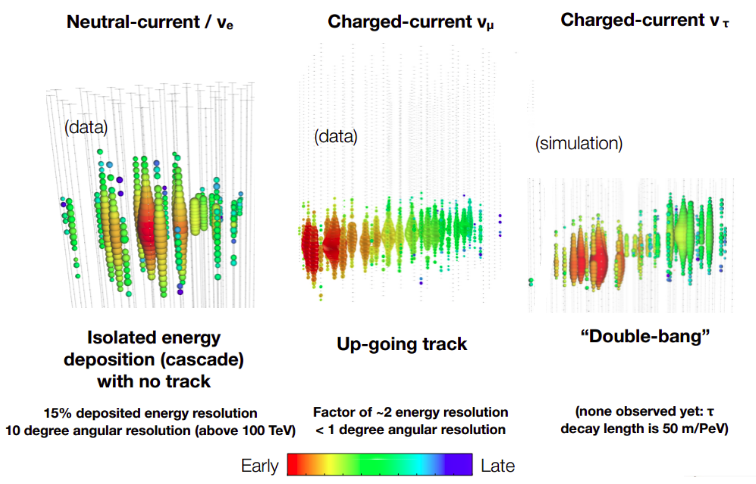
\includegraphics[width=\textwidth]{chapter4/img/ICinteractions2.png}
\caption{Neutrino interactions in the IceCube detector have two distinct types of interactions: cascades and tracks. Energetic taus are theorized to have double-bang signatures but have not undeniably been seen. Colors determine the timing of hits in the optical modules in the ice. Illustrations from the IceCube collaboration.}
\label{fig:ICinteractions2}
\end{figure}
 
\subsection{DeepCore}
A subset of in-ice DOMs is deployed along eight extra strings in the central region of the in-ice array. The optical modules are deployed deeper than 1750 meter with a denser instrumented volume. Seven strings of the standard IceCube strings are also combined with these strings to optimize the instrumented volume for this detector. The inter-string spacing on the eight specialized DeepCore strings varies from 41 m to 105 m. The DOM-to-DOM spacing is 7 m for the bottom 50 optical modules (which are deployed at depths of 2100 m to 2450 m). The remaining 10 DOMs on each string are located from depths shallower than 2000 m with a spacing of 10 m. This extra ``layer'' surves as a veto for downgoing atmospheric muons. In total, each strings is instrumented with 60 DOMs, resulting in a total of 480 DOMs. Instrumentation in the ice between 2000 m to 2100 proved to be less useful due to the \textit{dust layer} (see Section \cite{sec:ice}) and was therefore left out. Six out of the eight specialized strings are also instrumented with DOMs using PMTs of higher quantum efficiency. The two remaining strings are instrumented with regular IceCube DOMs.

The DeepCore design allows us to detect neutrinos of much lower energies in the range of $\mathcal{O}$(10 GeV)– $\mathcal{O}$(100 GeV). Experiments for neutrino oscillation experiments, WIMP dark matter annihilation, galactic supernova neutrinos and point sources are made possible or more feasible with this dense subarray \cite{Collaboration:2011ym}.

\subsection{IceTop}
IceTop is a cosmic ray air shower array, located on the surface of the ice and 2835 m above sea level. As discussed in Chapter \ref{ch:cr}, air showers die out when they are propagating to Earth's surface but as a consequence of the high altitude of IceTop, showers are observed near maximum resulting in a good energy resolution for the detector. This is important if one wants to measure changes in composition as a function of energy. In total, 162 ice-filled tanks are distributed across 81 stations (two tanks per station) in a similar grid on which the in-ice array is deployed. Similar to the denser DeepCore infill, there are eight stations in the center of IceTop placed more closely together. The two tanks per station are separated 10 m apart from each other and each tank contains two regular IceCube DOMs. One is operated at a ``low-gain'' and one at ``high-gain'', making them more fitted for air shower detection. The tanks measure the Cherenkov light that is produced in the ice of a tank due to the particles in a shower (electrons, positrons, muons and hadrons). The IceTop design allows to fully cover the knee of the energy spectrum and is primarily sensitive to PeV to EeV energies. The denser infill alows the threshold to be lowered to 100 TeV. The detector is used in studies of the composition, gammma rays, high-$p_T$ muons, etc. 

\subsection{IceCube Laboratory}
The central building to which the modules of all the detectors are connected is the IceCube Laboratory (ICL). Cables/strings from the arrays run are routed up two cable towers on either sides of the structure. An picture of the ICL is shown as the header image of this chapter, one of the towers is visible. Inside the main part of the building there is a server room to which the cables in the towers are connected (Section \ref{subsec:cablesystems}???). The server room is protected against electromagnetic interference with a metal mesh. All data acquisition and online filtering computers are housed inside the server room together with the main IceCube computing system called the ``'South Pole System' (Section ???). 
\section{Antarctic ice}
\label{sec:ice}
Relativistic particles travelling through the ice produce photons in a Cherenkov cone of around 41$^\circ$. How these photons propagate from the point of emission to the receiving sensors is determined by absorption and scattering within the ice. These propagation effects are important for both simulation and reconstruction of IceCube data requiring a good understanding of the underlying properties of the medium. The most important parameters necessary to describe the photon propagation in ice is: the average distance to absorption, the average distance between successive scatters of photons, and the angular distribution of the new direction of a photon at each given scattering point. There has been a large effort into measuring and modeling the Antarctic ice that is still ongoing. A good summary (which is a bit outdated) can be found in reference \cite{Aartsen:2013rt}.
\subsection{Ice simulation}
To be able to simulate the ice each DOM was instrumented with 12 LEDs aimed in six different azimuth angles (with 60$^\circ$ spacing) and along two different zenith angles. The LEDs were chosen to have a wavelength spectrum centered at around 400 nm to approximate the typical wavelength of detected Cherenkov photons.

The ice is modeled by the six-parameter ice model introduced in \cite{Ackermann:2006pva}. In this model the ice is described by a table of depth-dependent parameters $b_e(400)$ and $a_{dust}(400)$ related to scattering and absorption at a wavelength of 400 nm. These two parameters are described by a depth-dependent relative temperature $\delta \tau$ and six global parameters. The effective scattering coefficient $b_e = b \cdot \left( 1-\langle \cos \theta \rangle \right)$, where $b$ is the geometrical scattering coefficient that determines the average distance between successive scatters and $\theta$ is the deflection angle at each scatter. The absorption coefficient $a$ determines the average distance traveled by a photon before it is absorbed and is the sum of two components: one due to dust and the other a temperature dependent component for pure ice.

\begin{equation}
b_e(\lambda)  = b_e(400) \cdot \left( \frac{\lambda}{400}\right)^{-\alpha},
\end{equation}

\begin{equation}
a(\lambda) = a_{dust}(\lambda) + A e^{-B/\lambda} \cdot (1+0.01 \cdot \delta t), \ \ \ \textrm{with} \ \ \ a_{dust}(\lambda) = a_{dust}(400) \cdot \left( \frac{\lambda}{400}\right)^{-\kappa}.
\end{equation}
$\alpha, \kappa, A \textrm{and} B$ are determined in \cite{Ackermann:2006pva}\footnote{The remaining two parameters $D$ and $E$ were not used here.}, $\delta \tau$ is equal to

\begin{equation}
\delta \tau(d) = T(d) - T(1730 \textrm{m}), \ \ \ \textrm{with} \ \ \ T(d) = 221.5 - 0.00045319 \cdot d + 5.822 \cdot 10^{-6} \cdot d^2.
\end{equation}
Using flasher data with 400 nm wavelengths, it is possible to measure the values of $b_e(400)$ and $a_{dust}(400)$ at certain depths and use the six-parameter ice model to extrapolate scattering and absorption for other wavelengths. 

In 2008 a flasher run was launched where each DOM on string 63 was producing flashes. The layout of the detector at the time of the flasher run and results of fits to $b_{e}(400)$ and $a(400)$ vs. depth can be found in Figure \ref{fig:2008config}. At a depth between 2000 m and 2100 m a large increase in scattering and absorption is clearly visible. A \textit{dust layer}, presumably originating to volcanic ash is characterized by an increase of dust in the ice, responsible for the higher scattering and absorption factors.

\begin{figure}[ht]
\begin{minipage}{6in}
  \centering
  \raisebox{-0.5\height}{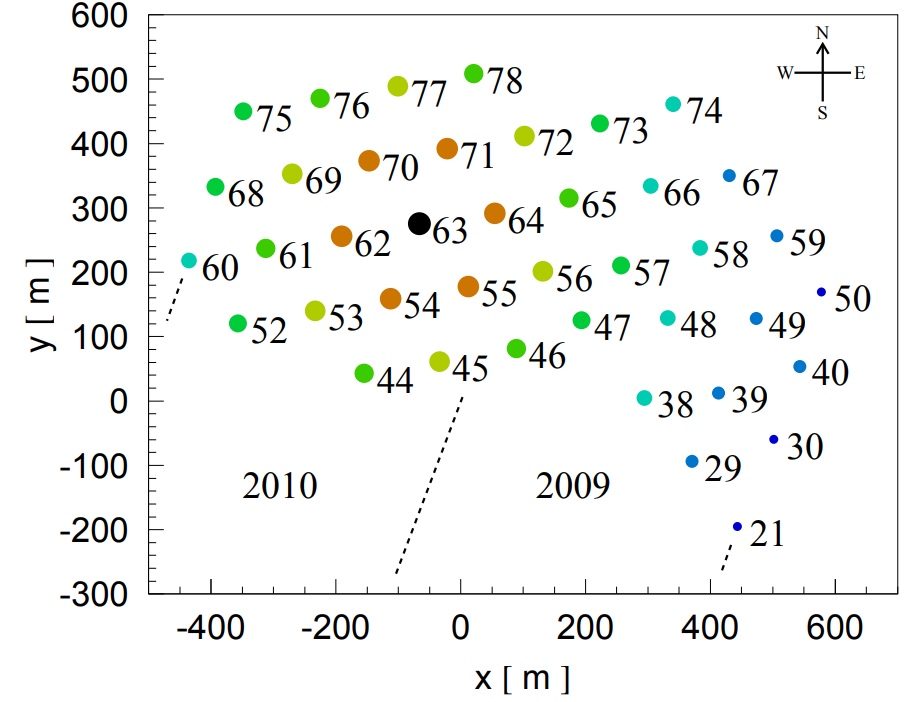
\includegraphics[height=2in]{chapter5/img/2008config.png}}
  \hspace*{.7in}
  \raisebox{-0.5\height}{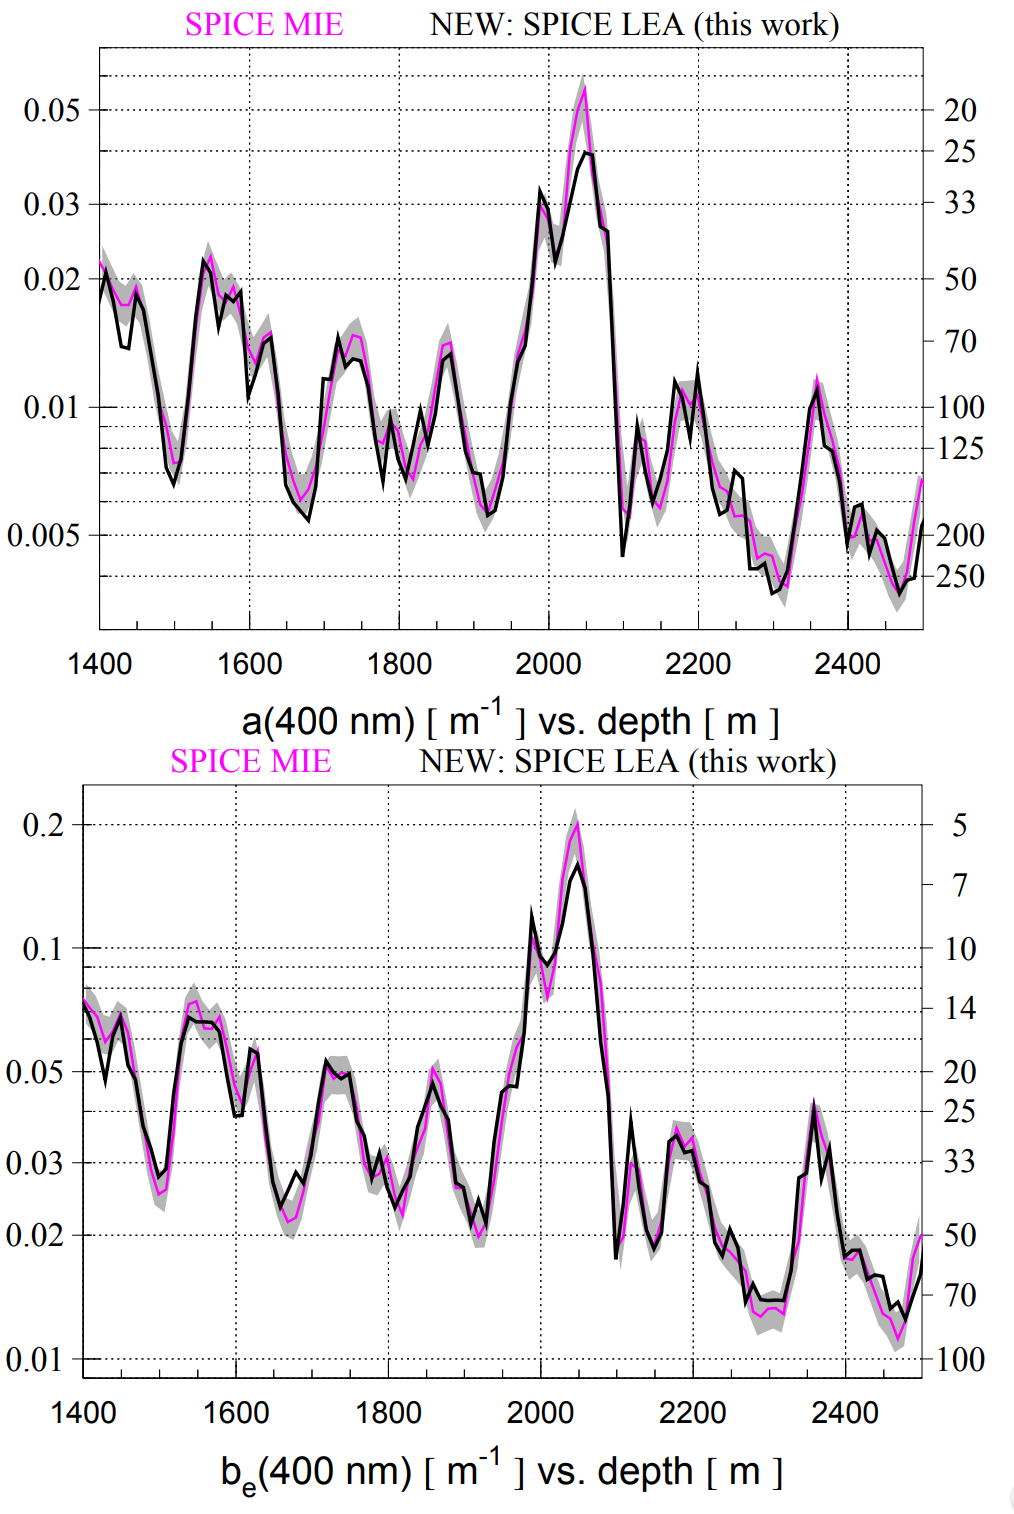
\includegraphics[height=3.5in]{chapter5/img/spiceleacoefficients.png}}
\end{minipage}
\caption{Left: Top view of the 2008 detector configuration when DOMs on string 63 were used to flash LEDs in a flasher run. Same colors are used for strings located at a similar distance to the central string. Right: values of $b_{e}(400)$ and $a(400)$ vs. depth for two different ice models. Both illustrations from \cite{1412998}.}
\stepcounter{figure}%
\label{fig:2008config}
\end{figure}

Over the years multiple different ice models have been constructed. For this analysis the SPICELea model has been set as nominal. This was the most recent model that had significant Monte Carlo background simulations available. It includes an angular sensitivity estimation according to the \textit{hole ice}, a column of ice approcimately 30 cm in radius immediately surrounding the strings with an increased amount of scattering\footnote{Hier uitleggen wat dit is}. More information about this model can be found in reference \cite{1412998}.
\subsection{Systematic uncertainties}
The complex nature of the characteristics of the ice such as the dust particles, the tilt in the ice sheets, etc. result into non-negligible uncertainties in tehe ice model. Data from the flasher runs are compared to simulation and this verification was used to quantify the uncertainty on the measured values of $b_e(400)$ and $a(400)$. From this, it was determined that $(+10\%,0), (0,+10\%)$ and $(-7.1\%,7.1\%)$ uncertainties on the scattering and absorption coefficients was a conservative estimation.

\section{Hardware Components}
\subsection{Digital Optical Modules}
\label{subsec:doms}
The Digital Optical Modules, or DOMs, in the ice convert light into electrical signals and have the necessary hardware installed to perform some basic processing of the electrical pulses. A downward facing 10''-diameter photomultiplier tube (PMT) is able to detect light produced by electrons or muons typically ranging from 10 GeV to 10 PeV and distances up to 500 m away. The high voltage of the PMTs is set at 2 kV, resulting in a gain of $10^7$. The amplitude of the resulting waveforms ranges from 1 mV up to and beyond the linearity limit of the PMT ($\tilde 2$ V) with width ranging from 12 ns to 1500 ns. This wide dynamic range of waveform characteristics are processed by onboard electronics: the main board and delay board. The main board controls all the devices in the DOM (high voltage power supply for the PMT, the flasher board and pressure, temperature and power supply voltage monitor sensors), digitizes the PMT waveforms, communicates with the data acquisition (DAQ) on the surface, houses an internal clock which is regularly calibrated with the DAQ on the surface and exchanges LC pulses with the adjacent DOMs (explained below).
An illustration on the mechanical components of the optical module and a schematic view of the data flow starting from the PMT is shown in Figure \ref{fig:DOM}.

\subsection{PMTs}
The 10'' (or 25 cm) diameter PMT \cite{Abbasi:2010vc}
Iets van wavelength dependence van Frank-Tamm:

\begin{equation}
\frac{dN}{dx} = \int_{\lambda_1}^{\lambda_2} \frac{2 \pi \alpha}{\lambda^2} \sin^2 \left(\theta_c\right) d\lambda = 2\pi \alpha \sin^2 \left(\theta_c\right) \left(\frac{1}{\lambda_1} -\frac{1}{\lambda_2}\right).
\end{equation}
The PMTs in the DOMs are most sensitive between 300-650 nm and from the formula above we can calculate that this have an expected rate of around 350 photons per cm for a Cherenkov emission profile.

\begin{figure}
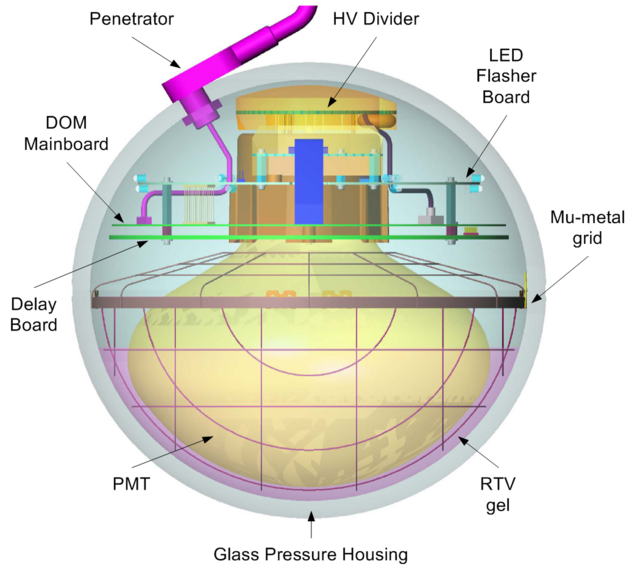
\includegraphics[width=0.48\textwidth]{chapter5/img/DOM-Picture.png}
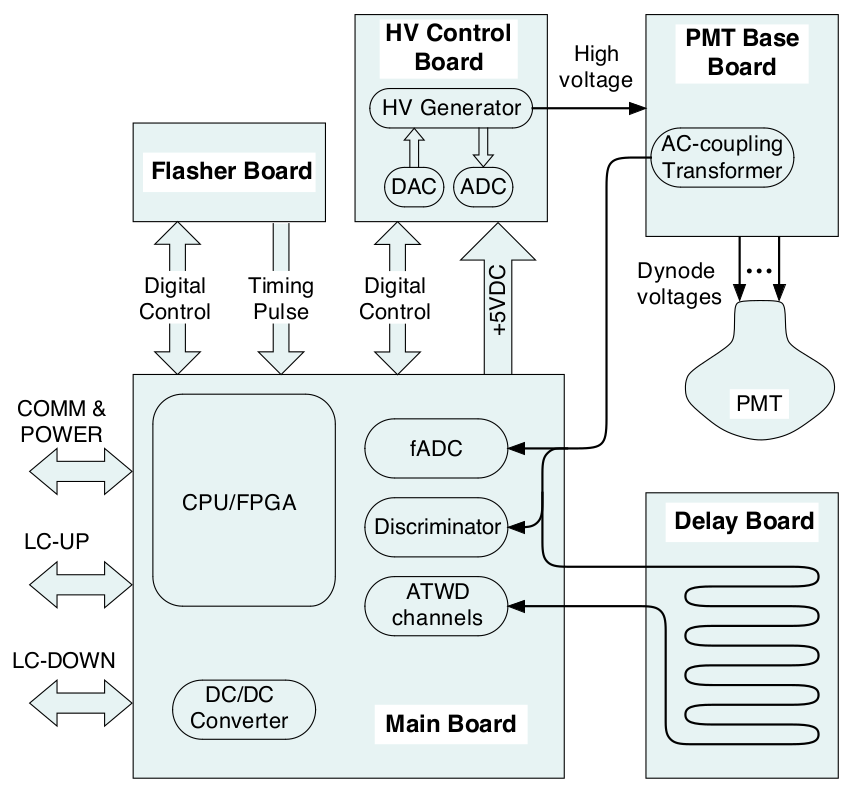
\includegraphics[width=0.48\textwidth]{chapter5/img/electronicsDOM.png}
\caption{\textit{Left:} illustrations of the mechanical DOM components. \textit{Right}: Scheme of the functional connections.}
\label{fig:DOM}
\end{figure}

Has to withstand enormous pressures and now still ... active

\subsection{Calibration Devices}
\subsection{Cable Systems}
\label{subsec:cablesystems}

\section{Deployment}

\section{Data Taking}

\section{Search Strategies}
\subsection{Astrophysical neutrinos}
\subsection{Point sources}
\subsection{Oscillations}
\subsection{Beyond The Standard Model Searches}

Ook de voornaamste zoektochten van IceCube vermelden en duiden. Bv de point sources, astrophysical (Sam zijn thesis bv) etc.

\section{Discussion}
?

\section{Future Upgrades}
Gen2 illustratie: \url{https://icecube.wisc.edu/~jkelley/talks/nnn18_kelley_icecube_detector_v1.pdf}






Copy paste van Wikipedia:
 Data from the Fermi Space Telescope (2013)[3] have been interpreted as evidence that a significant fraction of primary cosmic rays originate from the supernova explosions of stars.[4] Active galactic nuclei also appear to produce cosmic rays, based on observations of a neutrino and gamma rays from blazar TXS 0506+056 in 2018.[5][6]
 

\subsection{Muon tracks}
Ook muonen van atmosfeer, in hfdstk 4 enkel over muonen van neutrinos gebabbeld.
intro intro
The track-like structure of the signal allows to find a good ``lever arm'' as the deposited charge on the earliest and latest DOMs provide strong constraints on the event's position, time and direction. As a result, directional reconstruction..... Muons can transit the entire detector, making it difficult to reconstruct the energy of the muon and the parent neutrino. Starting muon tracks are challenging, but more useful to infer the initial energy of the neutrino. Highly relativistic muons are stochastic in nature and the energy loss depends on the energy of the particle. Using equation ??? it is possible to have a better energy reconstruction.
\subsection{Cascades}
The light output has a slight asymmetry in the direction of motion, making directional reconstructions challenging. However, these interactions are often calorimetric and therefore allow for nearly complete measurements of the energy and result in a good energy resolution.




Ook hoofdstuk 6 van: \url{https://edoc.hu-berlin.de/bitstream/handle/18452/17668/yanez-garza.pdf?sequence=1&isAllowed=y}